\chapter{Protótipo}
\label{apendice:prototipo}

As Figuras~\ref{p1} a~\ref{p9} apresentam o protótipo de alta fidelidade desenvolvido para o projeto, com base nos requisitos funcionais e não funcionais identificados nas Tabelas~\ref{tab:requisitosfunc} e~\ref{tab:requisitosnaofunc}, respectivamente.

\begin{figure}[H]
    \centering
    \caption{Tela Inicial.}
    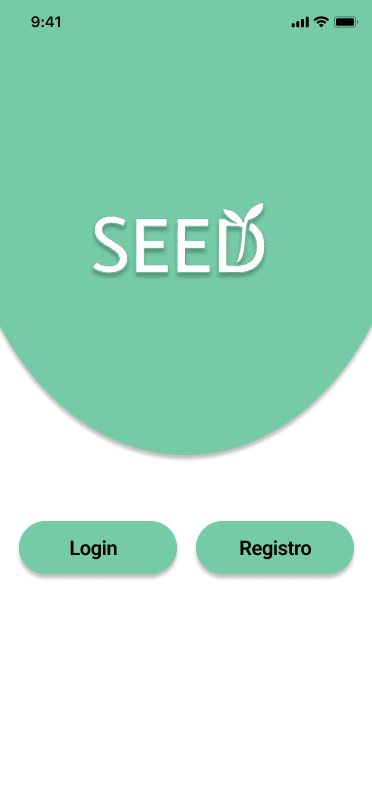
\includegraphics[height=0.7\textheight]{figuras/prototipo/i1.png}
    \par
    Fonte: autoria própria.
    \par
    \label{p1}
\end{figure}

\begin{figure}[H]
    \centering
    \caption{Tela de Login.}
    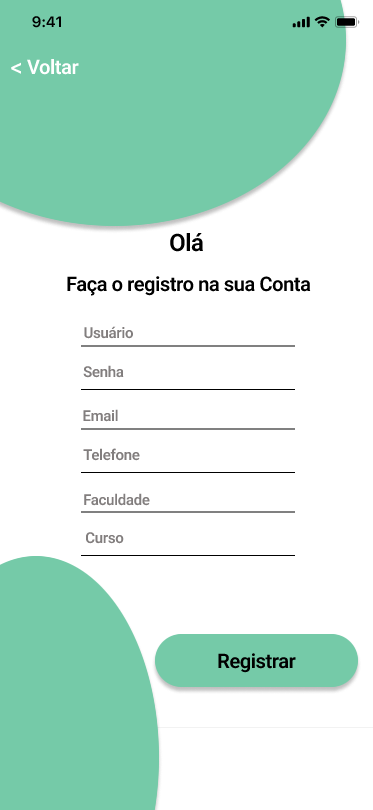
\includegraphics[height=0.4\textheight]{figuras/prototipo/i2.png}
    \par
    Fonte: autoria própria.
    \par
    \label{p2}
\end{figure}

\begin{figure}[H]
    \centering
    \caption{Tela de Registro.}
    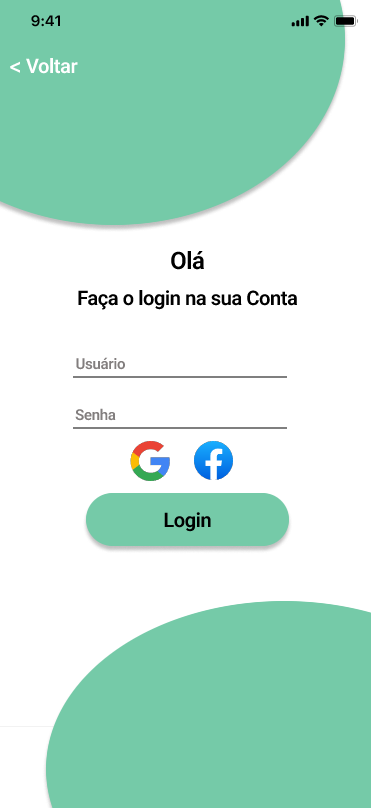
\includegraphics[height=0.4\textheight]{figuras/prototipo/i3.png}
    \par
    Fonte: autoria própria.
    \par
    \label{p3}
\end{figure}

\begin{figure}[H]
    \centering
    \caption{Tela de Resposta ao Formulário.}
    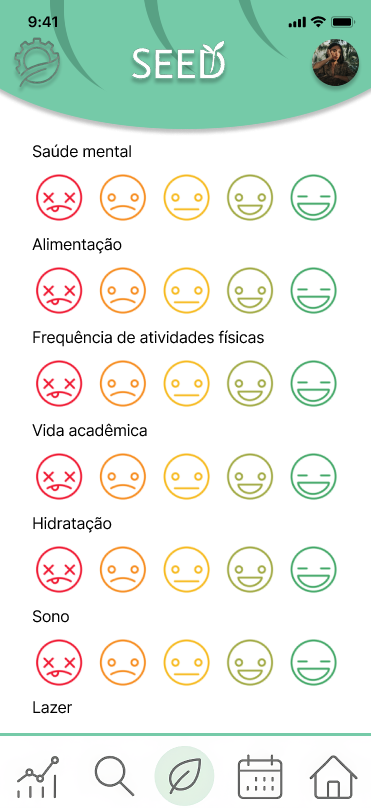
\includegraphics[height=0.4\textheight]{figuras/prototipo/i4.png}
    \par
    Fonte: autoria própria.
    \par
    \label{p4}
\end{figure}

\begin{figure}[H]
    \centering
    \caption{Tela de Alteração de Dados Pessoais.}
    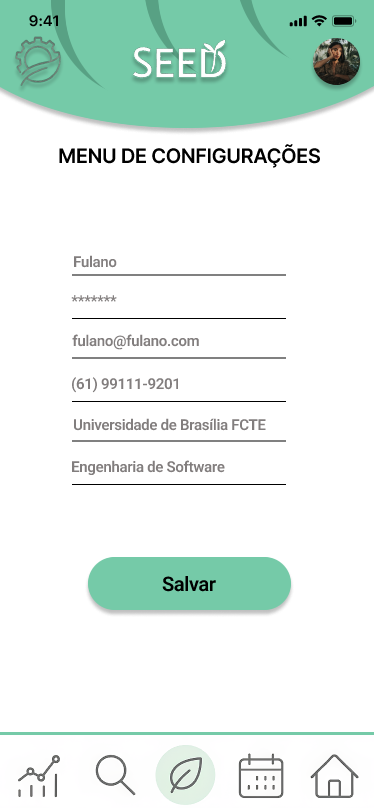
\includegraphics[height=0.4\textheight]{figuras/prototipo/i5.png}
    \par
    Fonte: autoria própria.
    \par
    \label{p5}
\end{figure}

\begin{figure}[H]
    \centering
    \caption{Tela FAQ}
    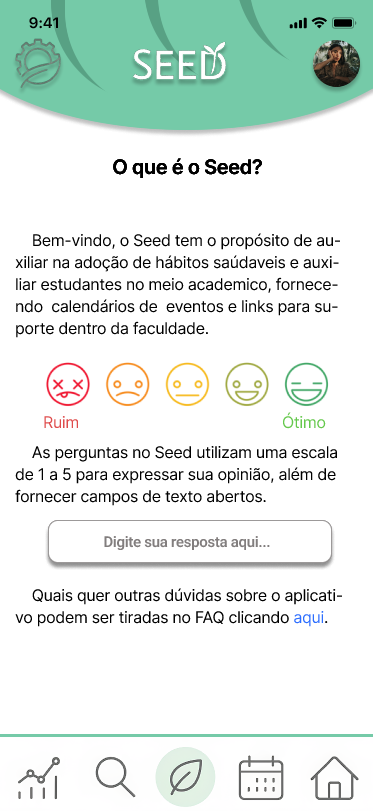
\includegraphics[height=0.4\textheight]{figuras/prototipo/i6.png}
    \par
    Fonte: autoria própria.
    \par
    \label{p6}
\end{figure}

\begin{figure}[H]
    \centering
    \caption{Tela de Estatísticas do Usuário.}
    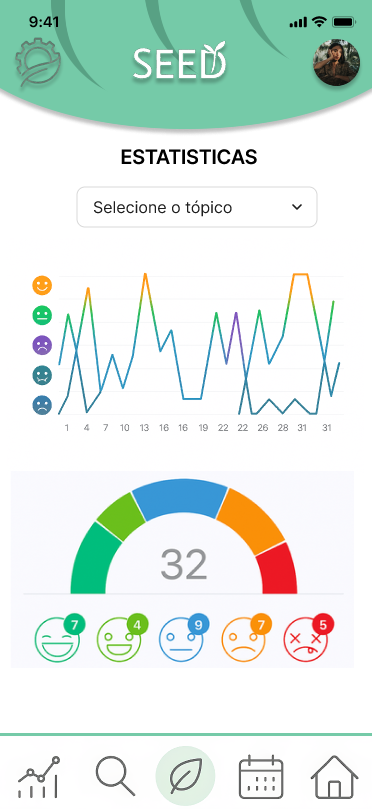
\includegraphics[height=0.4\textheight]{figuras/prototipo/i7.png}
    \par
    Fonte: autoria própria.
    \par
    \label{p7}
\end{figure}

\begin{figure}[H]
    \centering
    \caption{Tela do Calendário.}
    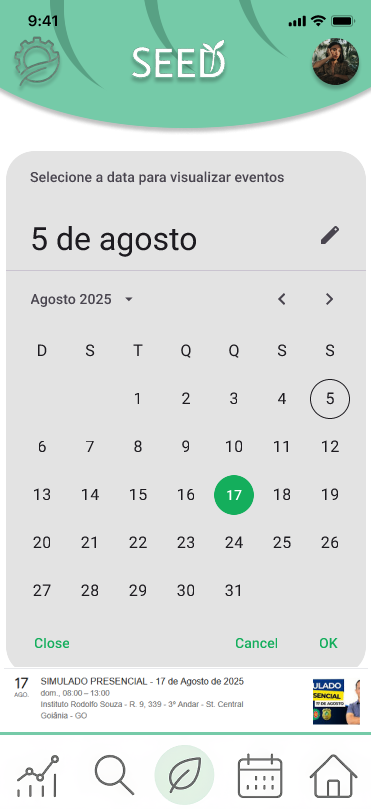
\includegraphics[height=0.4\textheight]{figuras/prototipo/i8.png}
    \par
    Fonte: autoria própria.
    \par
    \label{p8}
\end{figure}

\begin{figure}[H]
    \centering
    \caption{Tela do Feed de Eventos.}
    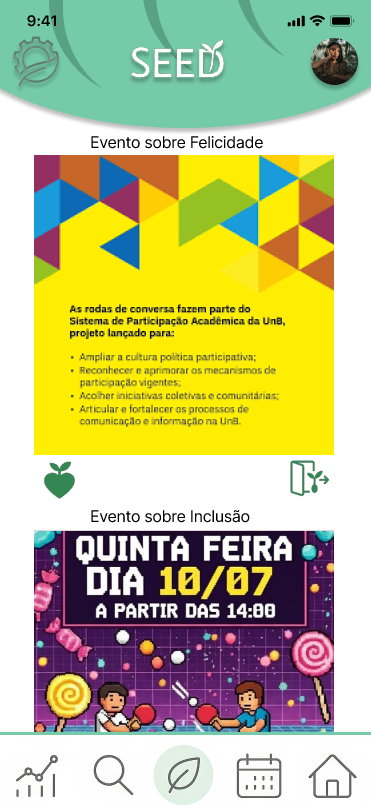
\includegraphics[height=0.4\textheight]{figuras/prototipo/i9.png}
    \par
    Fonte: autoria própria.
    \par
    \label{p9}
\end{figure}